\chapter{Capitolo 27}
\section{Il modello Bell-LaPadula per la sicurezza informatica}
\subsection{Modelli di sicurezza informatica}
In primo luogo, tutti i sistemi software complessi alla fine hanno rivelato difetti o bug che successivamente hanno dovuto essere corretti. Una buona discussione di questo può essere trovato nel classico The Mythical Man-Month. Secondo cui è straordinariamente difficile, se non impossibile, costruire un sistema hardware/software che non sia vulnerabile ad una varietà di attacchi alla sicurezza.

\singlespacing

I problemi per fornire una forte sicurezza del computer hanno coinvolto sia il design che l'implementazione. È difficile, progettare qualsiasi hardware o software, ed essere sicuri che il progetto fornisca di fatto il livello di sicurezza che è stato previsto. Questa difficoltà si traduce in molte vulnerabilità di sicurezza non previste. Anche se il progetto è in un certo senso corretto, è difficile, se non impossibile, implementare il progetto senza errori o bug, fornendo un'altra serie di vulnerabilità. Questi problemi hanno portato al desiderio di sviluppare un metodo per dimostrare, logicamente o matematicamente, che un particolare progetto soddisfa un insieme dichiarato di requisiti di sicurezza e che l'implementazione di quel progetto è fedelmente conforme alle specifiche del progetto.

\singlespacing

A tal fine, i ricercatori di sicurezza hanno cercato di sviluppare modelli formali di sicurezza del computer che possono essere utilizzati per verificare i progetti e le implementazioni di sicurezza.

\singlespacing

Inizialmente, la ricerca in questo settore è stata finanziata dal Dipartimento della Difesa degli Stati Uniti e sono stati fatti notevoli progressi nello sviluppo di modelli e nella loro applicazione a sistemi prototipo. Quel finanziamento è notevolmente diminuito così come i tentativi di costruire modelli formali di sistemi complessi. Il modello di sicurezza informatica più influente il modello Bell-LaPadula (BLP).

\subsection{Descrizione Generale}
Il modello BLP è stato sviluppato negli anni '70 come modello formale per il controllo degli accessi. Il modello modello si basava sul concetto di controllo dell'accesso. Nel modello, ad ogni soggetto e ad ogni oggetto viene assegnata una classe di sicurezza. Nella formulazione più semplice formulazione, le classi di sicurezza formano una rigida gerarchia e sono chiamate livelli di sicurezza.

\singlespacing

Un esempio è lo schema di classificazione militare degli Stati Uniti:

\begin{center}
    \textbf{top secret $>$ secret $>$ confidential $>$ restricted $>$ unclassified}
\end{center}

È possibile anche aggiungere un insieme di compartimenti, o categorie, ad ogni livello di sicurezza, così che un soggetto deve essere assegnato sia al livello appropriato che al compartimento per accedere ad un oggetto. Questo concetto è ugualmente applicabile in altre aree, dove le informazioni possono essere organizzate in livelli vuoti e scompartimenti pieni, e agli utenti possono essere concesse autorizzazioni per accedere a certi compartimenti di dati. Per esempio, il livello più alto di sicurezza potrebbe essere per i documenti ed i dati strategici di pianificazione aziendale, accessibili solo ai funzionari aziendali e al loro staff.

\singlespacing

Questo suggerisce uno schema di classificazione:

\begin{center}
    \textbf{strategic $>$ sensitive $>$ confidential $>$ public}
\end{center}

\begin{itemize}

    \item Un soggetto ha un nulla osta di sicurezza di un determinato livello
    
    \item Un oggetto deve avere una classificazione di sicurezza di un determinato livello.
    
\end{itemize}

Le classi di sicurezza controllano il modo con cui un soggetto può accedere ad un oggetto. Il modello ha definito quattro modalità di accesso.

\singlespacing

I modi sono i seguenti:

\begin{enumerate}
    \item \textbf{Lettura:}
    Al soggetto è permesso solo l'accesso in lettura all'oggetto.
    
    \item \textbf{Append:}
    Al soggetto è permesso solo l'accesso in scrittura all'oggetto.
    
    \item \textbf{Scrittura:}
    Il soggetto è autorizzato ad accedere sia in lettura che in scrittura all'oggetto.
    
    \item \textbf{Esecuzione:}
    Il soggetto non è autorizzato né a leggere né a scrivere sull'oggetto ma può invocare l'oggetto per l'esecuzione.
\end{enumerate}

Quando vengono definite più categorie o livelli di dati, il requisito viene definito sicurezza multilivello (MLS). La dichiarazione generale del requisito per la sicurezza multilivello incentrata sulla riservatezza è che un soggetto ad un livello alto non può trasmettere informazioni ad un soggetto ad un livello inferiore a meno che quel flusso rifletta accuratamente la volontà di un utente autorizzato come rivelato da una declassificazione autorizzata. Ai fini dell'implementazione, questo requisito è in due parti ed è dichiarato semplicemente.

\singlespacing

Un sistema sicuro multilivello per la riservatezza deve far rispettare quanto segue:

\begin{itemize}
    \item \textbf{Nessuna lettura:} Un soggetto può leggere solo un oggetto di livello di sicurezza inferiore o uguale. Questo è indicato in letteratura come la proprietà di sicurezza semplice (ss-property).
    
    \item \textbf{Nessuna scrittura:} Un soggetto può solo scrivere in un oggetto di livello di sicurezza maggiore o uguale. Questo è indicato in letteratura come la proprietà1 (pronunciato star property).
\end{itemize}

\begin{figure}[H]
	\centering
    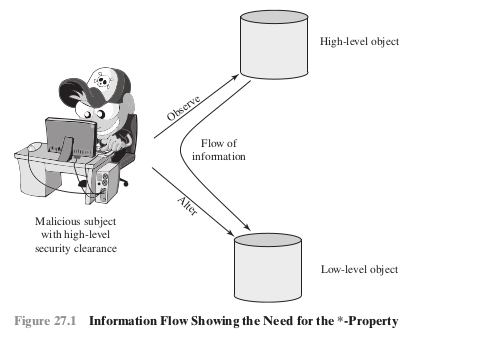
\includegraphics[width=12cm, keepaspectratio]{Bistarelli/img/cap_27/figura27.1.png}
\end{figure}

Qui, un soggetto malintenzionato passa informazioni classificate mettendole in un contenitore di informazioni etichettato con una classificazione di sicurezza inferiore a quella delle informazioni stesse. Questo permetterà un successivo accesso in lettura a queste informazioni da parte di un soggetto con un livello di autorizzazione inferiore. Queste due proprietà forniscono la forma di riservatezza di ciò che è noto come controllo obbligatorio dell'accesso (MAC). Sotto il MAC, non è permesso alcun accesso che non soddisfi queste due proprietà. Inoltre, il modello BLP prevede un controllo di accesso discrezionale (DAC).
\begin{itemize}
    \item \textbf{DS-propietà}
    
    Un individuo (o ruolo) può concedere a un altro individuo (o ruolo) l'accesso a un documento in base alla discrezione del proprietario, limitato dalle regole MAC regole.


Così, un soggetto può esercitare solo gli accessi per i quali ha la necessaria autorizzazione e che soddisfano le regole del MAC.
\end{itemize}
\subsection{Descrizione formale del modello}
Il modello si basa sul concetto di uno stato attuale del sistema. Lo stato è descritto dalla 4-tupla (b, M, f, H), definita come segue:
\begin{itemize}
    \item \textbf{Insieme di accesso corrente b:}
    
    Questo è un insieme di triple della forma (soggetto, oggetto, accesso-modo). Una tripla (s, o, a) significa che il soggetto s ha accesso corrente a o nel modo di accesso a. Questo non significa semplicemente che s ha il diritto di accesso ad a o ad o. La tripla significa che s sta attualmente esercitando tripla significa che s sta attualmente esercitando quel diritto di accesso; cioè, s sta attualmente accedendo ad a o in modalità a.
    
    \item \textbf{Matrice di accesso M:}
    
    L'elemento della matrice Mij registra le modalità di accesso in cui il soggetto Si è autorizzato di accedere all'oggetto Oj.
    
    \item \textbf{Funzione di livello F:}
    
    Questa funzione assegna un livello di sicurezza ad ogni soggetto e oggetto. Consiste di tre mappature: fo(Oj) è il livello di classificazione dell'oggetto Oj e fs(Si) che è il nulla osta di sicurezza del soggetto Si. fc(Si) è il livello di sicurezza attuale del soggetto Si. Il nulla osta di sicurezza di un soggetto è il massimo livello di sicurezza del soggetto. Il soggetto può operare a questo livello o a un livello inferiore. Così, un utente può accedere al sistema ad un livello inferiore al nulla osta di sicurezza dell'utente. Questo è particolarmente utile in un sistema di controllo dell'accesso basato sui ruoli.
    
    \item \textbf{Gerarchia H:}
    
    Si tratta di un albero con radici dirette i cui nodi corrispondono agli oggetti del sistema. Il modello richiede che il livello di sicurezza di un oggetto domini il livello di sicurezza del suo genitore. Per la nostra discussione, possiamo equiparare questo, alla condizione che il livello di sicurezza di un oggetto deve essere maggiore o uguale al suo genitore.
\end{itemize}

\newpage
Possiamo ora definire le tre proprietà di BLP in modo più formale. Per ogni soggetto Si e ogni oggetto Oj, i requisiti possono essere dichiarati come segue:

\begin{itemize}
    \item \textbf{ss-property:} Tutte le triple della forma (Si, Oj, read) nell'insieme corrente di accesso b hanno la propietà fc(Si) $>=$ fo(Oj).
    
    \item \textbf{property:} Tutte le triple della forma (Si, Oj, append) nell'insieme di accesso corrente b ha la propietà fc(Si) $<=$ fo(Oj). Tutte le triple della forma (Si, Oj, write) nell'attuale set di accesso b hanno la propietà fc(Si) $=$ fo(Oj).
    
    \item \textbf{ds-property:} Se (Si, Oj, Ax) è un'accesso corrente (in b), la modalità di accesso Ax è registarta in (Si, Oj) elemnti di M. Questo da (Si, Oj, Ax) ed implica che Ax $\in$ M\[Si, Oj\].

\end{itemize}
Queste tre proprietà possono essere utilizzate per definire un sistema sicuro per la riservatezza.

\singlespacing

In sostanza, un sistema sicuro è caratterizzato da quanto segue:
\begin{enumerate}
    \item Lo stato di sicurezza attuale del sistema (b, M, f, H) è sicuro se e solo se ogni elemento di b soddisfa le tre proprietà.
    
    \item Lo stato di sicurezza del sistema viene cambiato da qualsiasi operazione che causa un cambiamento uno qualsiasi dei quattro componenti del sistema, (b, M, f, H).
    
    \item Un sistema sicuro rimane sicuro finché qualsiasi cambiamento di stato non viola le tre proprietà.
\end{enumerate}
Questi tre punti possono essere espressi come teoremi usando il modello formale. Inoltre, dato un progetto o un'implementazione attuale, è teoricamente possibile dimostrare che il sistema è sicuro provando che ogni azione che influisce sullo stato del sistema soddisfa le tre proprietà. In pratica, per un sistema complesso, tale prova non è mai stata completamente sviluppata. Tuttavia, come menzionato prima, la dichiarazione formale dichiarazione formale dei requisiti può portare ad una progettazione e implementazione più sicura.

\newpage
\subsection{Operazioni Astratte}
Il modello BLP include un insieme di regole basate su operazioni astratte che cambiano lo stato del sistema. Le regole sono le seguenti:

\begin{enumerate}
    \item \textbf{Ottenere l'accesso}
    
    Aggiungere una tripla (soggetto, oggetto, modalità di accesso) al set di accesso corrente b. Utilizzato da un soggetto per avviare l'accesso a un oggetto nel modo richiesto

    \item \textbf{Rilasciare l'accesso}
    
    Rimuove una tripla (soggetto, oggetto, modo di accesso) dal set di accesso corrente b. Usato per rilasciare un accesso precedentemente iniziato.
    
    \item \textbf{Cambiare livello dell'oggetto}
    
    Cambia il valore di fo(Oj) per qualche oggetto Oj. Usato da un soggetto per modificare il livello di sicurezza di un oggetto
    
    \item \textbf{Cambiare livello attuale}
    
    Cambia il valore di fc(Si) per qualche soggetto Si. Usato da un soggetto per alterare il livello di sicurezza di un oggetto.
    
    \item \textbf{Dare il permesso di accesso}
    
    Aggiungere una modalità di accesso a qualche voce della permissione M. Usato da un soggetto per concedere un modo di accesso su un oggetto specificato a un altro soggetto.
    
    \item \textbf{Rescindere il permesso di accesso}
    
    Cancella un modo di accesso da qualche voce di M. Usato da un soggetto per revocare un accesso precedentemente concesso.
    
    \item \textbf{Creare oggetto}
    
    Attacca un oggetto alla struttura ad albero corrente H come foglia. Usato per creare un nuovo oggetto o attivare un oggetto che è stato precedentemente definito ma è inattivo perché non è stato inserito in H.
    
    \item \textbf{Cancellare un gruppo di oggetti}
    
    Stacca da H un oggetto e tutti gli altri oggetti sotto di esso nella gerarchia. Questo rende il gruppo di oggetti inattivo. Questa operazione può anche modificare l'attuale set di accesso b perché tutti gli accessi all'oggetto vengono rilasciati.
\end{enumerate}

Le regole 1 e 2 alterano l'accesso corrente. Le regole 3 e 4 alterano le funzioni di livello. Le regole 5 e 6 alterano il permesso di accesso e le regole 7 e 8 alterano la gerarchia. Ogni regola è governata dall'applicazione delle tre proprietà. Per esempio, per ottenere l'accesso per una lettura, dobbiamo avere $fc(Si) >= fo(Oj)$ e $Ax \in M[Si, Oj]$.

\subsection{Esempio di utilizzo Bella-Pabula}
Questo esempio illustra il funzionamento del modello BLP ed evidenzia anche un problema pratico problema pratico che deve essere affrontato. Assumiamo un sistema di controllo degli accessi basato sui ruoli. 

\singlespacing

Carla e Dirk sono utenti del sistema. Carla è una studentessa (s) nel corso c1. Dirk è un insegnante (t) nel corso c1, ma può anche accedere al sistema come studente; così, due ruoli sono assegnati a Dirk:

\begin{center}
    $Carla: (c1-s)$\\
    $Dirk: (c1-t), (c1-s)$
\end{center}

Al ruolo di studente è assegnato un nulla osta di sicurezza inferiore e al ruolo di insegnante un autorizzazione di sicurezza più alta. Vediamo alcune possibili azioni:

\begin{enumerate}
    \item \textbf{Dirk crea un nuovo file f1 come c1-t; Carla crea il file f2 come c1-s (vedi Figura 27.2a)}.
    
Carla può leggere e scrivere su f2, ma non può leggere f1, perché è a un livello di classificazione più alto (livello insegnante).

    \item \textbf{Nel ruolo c1-t, Dirk può leggere e scrivere f1 e può leggere f2 se Carla concede l'accesso a f2}. 
    
Tuttavia, in questo ruolo, Dirk non può scrivere f2 a causa della proprietà. Né Dirk né un cavallo di Troia per suo conto possono declassare i dati dal livello dell'insegnante al livello dello studente.

\singlespacing

Solo se Dirk si collega come studente può creare un file c1-s o scrivere su un file c1-s esistente, come f2. Nel ruolo di studente, Dirk può anche leggere f2.

    \item \textbf{Dirk legge f2 e vuole creare un nuovo file con commenti a Carla come feed-back}.

Dirk deve firmare nel ruolo studente c1-s per creare f3 in modo che sia accessibile da Carla (vedi Figura 27.2b). In un ruolo di insegnante, Dirk non può creare un file a livello di classificazione studente.

    \item \textbf{Dirk crea un esame basato su un file modello esistente memorizzato a livello c1-t}.
    
Dirk deve accedere come c1-t per leggere il modello, e anche il file che crea (f4) deve essere a livello dell'insegnante (vedi Figura 27.2c).

    \item \textbf{Dirk vuole che Carla faccia l'esame, e quindi deve fornirle un accesso in lettura}.
    
Tuttavia, tale accesso violerebbe la proprietà ss. Dirk deve declassare la classificazione di f4 da c1-t a c1-s.

\singlespacing

Dirk non può farlo nel ruolo c1-t perché questo violerebbe la proprietà. Pertanto, un amministratore di sicurezza (possibilmente Dirk in questo ruolo) deve avere l'autorità di downgrade e deve essere in grado di eseguire il downgrade al di fuori del modello BLP. La linea tratteggiata nella Figura 27.2d che collega f4 con c1-s-read indica che questa connessione non è stata generata dalle regole predefinite di BLP ma da un'operazione di sistema.

    \item \textbf{Carla scrive le risposte all'esame in un file f5}. 
    
Crea il file a livello c1-t in modo che solo Dirk possa leggere il file.

\singlespacing

Questo è un esempio di scrittura, che non è vietato dalle regole BLP. Carla può ancora vedere le sue risposte alla sua stazione di lavoro, ma non può accedere a f5 per leggere.
\end{enumerate}

\newpage
\begin{figure}[H]
	\centering
    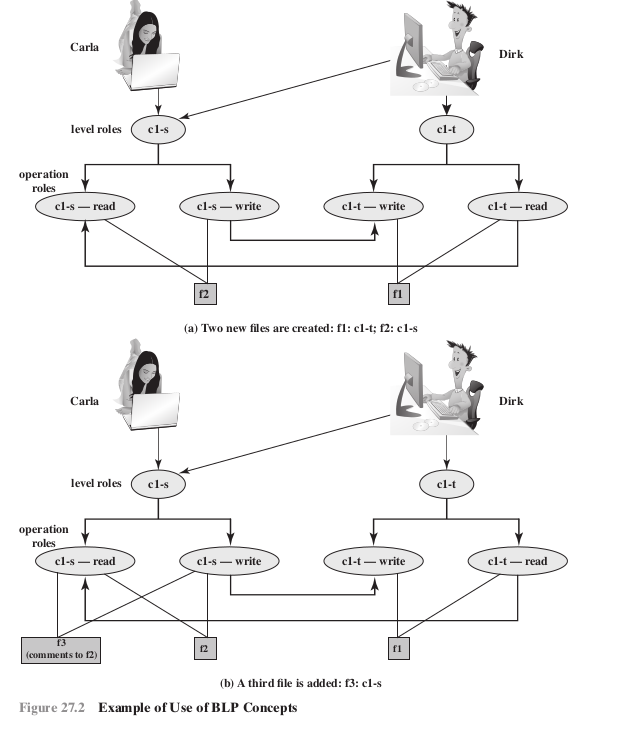
\includegraphics[width=10cm, keepaspectratio]{Bistarelli/img/cap_27/figura27.2.png}
\end{figure}

\begin{figure}[H]
	\centering
    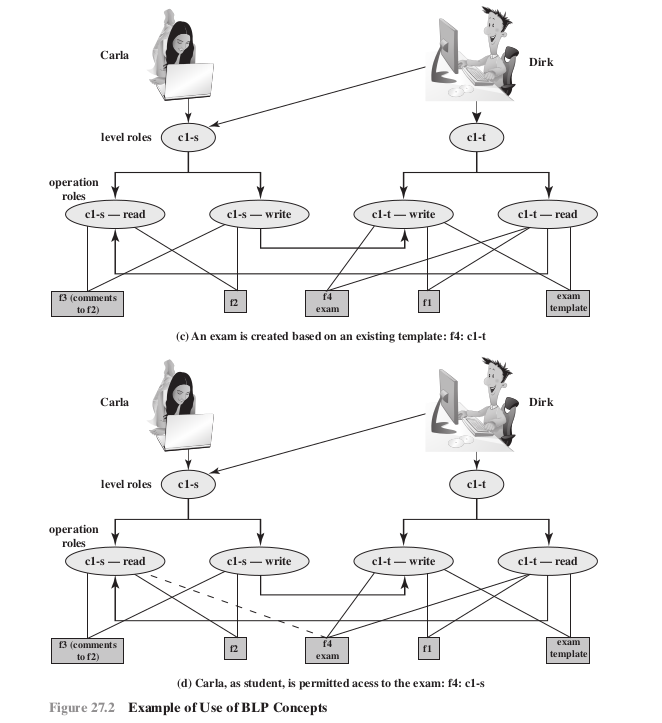
\includegraphics[width=10cm, keepaspectratio]{Bistarelli/img/cap_27/figura27.2b.png}
\end{figure}

\begin{figure}[H]
	\centering
    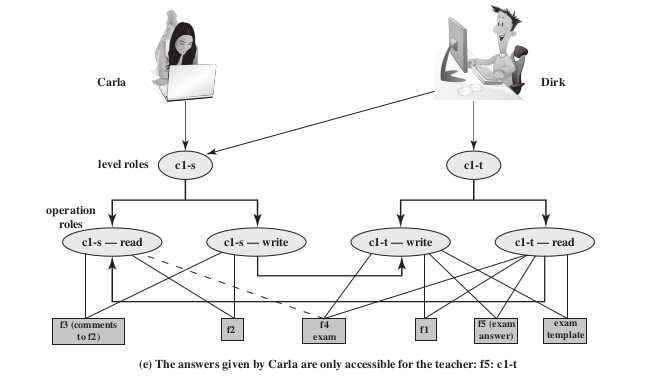
\includegraphics[width=10cm, keepaspectratio]{Bistarelli/img/cap_27/27.2c.png}
\end{figure}


In primo luogo, come notato al punto 4, il modello BLP non ha alcuna disposizione per gestire il "downgrade" di oggetti, anche se i requisiti per la sicurezza multilivello riconoscono che tale un flusso di informazioni da un livello superiore a uno inferiore può essere richiesto, purché rifletta la volontà di un utente autorizzato. Quindi, qualsiasi implementazione pratica di un sistema multilivello deve supportare tale processo in modo controllato e monitorato. Collegato a questo c'è un'altra preoccupazione. Un soggetto vincolato dal modello BLP può solo "editare" (leggere e scrivere) un file ad un livello di sicurezza mentre visualizza anche file allo stesso livello o a livelli inferiori. Se il nuovo documento consolida informazioni da una gamma di fonti e livelli, alcune di quelle informazioni sono ora classificate ad un livello rispetto a quello originale. Questo è noto come classification creep ed è un problema ben noto preoccupazione quando si gestiscono informazioni multilivello. Anche in questo caso, è necessario un processo di declassamento delle informazioni è necessario per ripristinare livelli di classificazione ragionevoli.
\newpage
\subsection{Esempio di implementazione Multics}
Un'implementazione di MLS sul sistema operativo Multics.

\singlespacing

Iniziamo con una breve descrizione degli aspetti rilevanti di Multics. Multics è un sistema operativo a tempo condiviso che fu sviluppato da un gruppo del MIT noto come Progetto MAC (computer ad accesso multiplo) negli anni '60. Multics era non solo anni, ma decenni in anticipo sui tempi. Anche a metà degli anni '80, quasi 20 anni dopo essere diventato operativo, Multics aveva caratteristiche di sicurezza superiori e una maggiore sofisticazione nell'interfaccia utente e in altre aree rispetto ad altri sistemi operativi per mainframe contemporanei. Sia la gestione della memoria che il file system in Multics sono basati sul concetto di segmenti. La memoria virtuale è segmentata. Ogni file nel file system è definito come un segmento. Così, il sistema operativo utilizza lo stesso meccanismo per caricare un segmento di dati dalla memoria virtuale nella memoria principale, e per caricare un file dalla memoria virtuale nella memoria principale. I segmenti sono organizzati gerarchicamente, da una directory principale fino ai singoli segmenti.

\singlespacing

Multics gestisce lo spazio di indirizzamento virtuale per mezzo di un segmento descrittore, che è associato ad un processo e che ha una voce per ogni segmento nella memoria virtuale accessibile da questo processo. Il registro base del segmento del descrittore punta all'inizio del segmento descrittore per il processo attualmente in esecuzione. Per MLS, sono necessarie due caratteristiche aggiuntive. Una tabella a livello di processo include ed una voce per ogni processo attivo, e la voce indica l'autorizzazione di sicurezza del processo. Associato ad ogni segmento c'è un livello di sicurezza, che è memorizzato nel segmento del segmento in questione.

\begin{figure}[H]
	\centering
    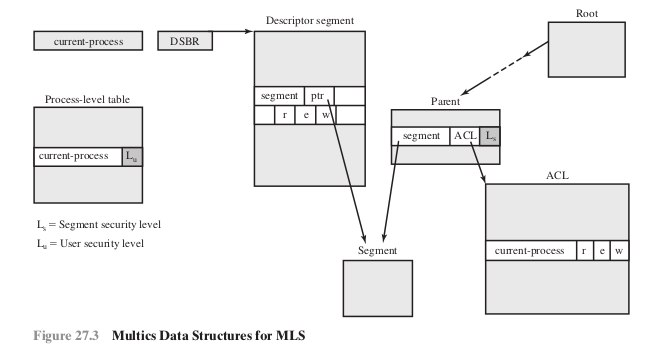
\includegraphics[width=10cm, keepaspectratio]{Bistarelli/img/cap_27/27.3.png}
\end{figure}


Corrispondente allo stato di sicurezza del modello BLP (b, M, f, H) è un insieme di strutture dati Multics (vedi Figura 27.3).

La corrispondenza è la seguente:

\begin{itemize}
    \item \textbf{b:} Segmento descrittore parola.
    
    Il segmento descrittore identifica il soggetto (processo). Il puntatore di segmento nella parola descrittore di segmento identifica l'oggetto (segmento dati). I tre bit di controllo dell'accesso nel segmento descrittore di segmento identificano il modo di accesso.
    
    \item \textbf{M:} elenco di controllo dell'accesso
    
    \item \textbf{f:} Informazioni nel segmento directory e nella tabella a livello di processo.
    
    \item \textbf{H:} Struttura gerarchica del segmento.

\end{itemize}

Con queste strutture di dati, Multics può imporre il controllo di accesso discrezionale e obbligatorio. Quando un processo tenta un accesso ad un segmento, deve avere il permesso di accesso desiderato come specificato dalla lista di controllo degli accessi. Inoltre, la sua autorizzazione di sicurezza viene confrontata con la classificazione di sicurezza del segmento a cui accedere per determinare se la regola di sicurezza semplice e la regola di sicurezza sono soddisfatte.

\subsection{Limitazioni modello BLP}
Mentre il modello BLP potrebbe, in teoria, porre le basi per un calcolo sicuro all'interno di un ambiente di amministrazione singola, ci sono alcune importanti limitazioni alla sua usabilità e difficoltà di implementazione.

\begin{enumerate}
    \item L'incompatibilità di riservatezza e integrità all'interno di un singolo sistema MLS. 
    
    In termini generali, MLS può funzionare sia per i poteri che per i segreti, ma non prontamente per entrambi. Questa esclusione reciproca esclude alcune interessanti tecnologie centrate sulla potenza e sull'integrità di essere usate efficacemente in ambienti MLS in stile BLP.
    
    \item Limitazione all'usabilità è il cosiddetto problema del cospiratore cooperante.
    
    In presenza di canali nascosti. In presenza di risorse condivise, la proprietà * può diventare inapplicabile. Questo è un problema specialmente nella presen contenuto attivo che è prevalente nell'attuale elaborazione di testi e in altri formati di documenti. Un documento maligno potrebbe contenere un soggetto che quando eseguito trasmette documenti classificati usando canali segreti a risorse condivise. In essenza, il modello BLP si rompe efficacemente quando i dati eseguibili (non fidati) a bassa classificazione dati eseguibili a bassa classificazione possono essere eseguiti da un soggetto ad alta autorizzazione (fidato).
\end{enumerate}

\newpage
\section{Altri modelli per la sicurezza informatica}
È importante notare che i modelli descritti in questo capitolo si concentrano sulla riservatezza o sull'integrità, con l'eccezione del Chinese Wall Model. L'incompatibilità delle preoccupazioni di riservatezza e integrità è riconosciuta come una grande limitazione all'usabilità di MLS in generale, e a MLS focalizzati sulla riservatezza in particolare.

\subsection{Modello di integrità Biba}

Il modello BLP si occupa della riservatezza ed è preoccupato della divulgazione non autorizzata delle informazioni. Il modello Biba si occupa dell'integrità e si occupa della modifica non autorizzata dei dati. Il modello Biba è destinato a trattare il caso in cui ci sono dati che devono essere visibili agli utenti a più o a tutti i livelli di sicurezza, ma devono essere modificati solo in modi controllati da agenti autorizzati.

\singlespacing

Gli elementi di base del modello Biba hanno la stessa struttura del modello BLP. Come con BLP, il modello Biba si occupa di soggetti e oggetti. Ogni soggetto e oggetto è assegnato un livello di integrità, indicato come I(S) e I(O) per il soggetto S e l'oggetto O, rispettivamente. Si può usare una semplice classificazione gerarchica, in cui c'è un ordine rigoroso dei livelli dal più basso al più alto.

\singlespacing

Come nel modello BLP, è anche possibile aggiungere un insieme di compartimenti allo schema di classificazione. 

\singlespacing

Il modello considera le seguenti modalità di accesso:

\begin{enumerate}
    \item \textbf{Modificare:} Scrivere o aggiornare le informazioni in un oggetto
    
    \item \textbf{Osservare:} Leggere le informazioni di un oggetto
    
    \item \textbf{Eseguire:} Eseguire un oggetto
    
    \item \textbf{Invocare:} Comunicazione da un oggetto all'altro
\end{enumerate}
I primi tre modi sono analoghi ai modi di accesso BLP. Il modo invoke è nuovo. Biba propone poi una serie di politiche alternative che possono essere imposte a questo modello. La più rilevante è la politica di integrità rigorosa, basata sulle seguenti regole:

\begin{itemize}
    \item \textbf{Integrità semplice:} Un soggetto può modificare un oggetto solo se il livello di integrità del soggetto domina il livello di integrità dell'oggetto: $I(S) >= I(O)$.
    
    \item \textbf{Confinamento dell'integrità:} Un soggetto può leggere un oggetto solo se il livello di integrità del soggetto è dominato dal livello di integrità dell'oggetto: $I(S) <= I(O)$.
    
    \item \textbf{Proprietà di invocazione:} Un soggetto può invocare un altro soggetto solo se il livello di integrità livello di integrità del primo soggetto domina il livello di integrità del secondo soggetto: $I(S1) >= I(S2)$.

\end{itemize}

Le prime due regole sono analoghe a quelle del modello BLP ma riguardano dell'integrità e invertono il significato di lettura e scrittura. La semplice regola di integrità è la restrizione logica di scrittura che impedisce la contaminazione dei dati ad alta integrità.
Un processo a bassa integrità può leggere dati a bassa integrità ma gli viene impedito di contaminare un file ad alta integrità con quei dati grazie alla semplice regola di integrità. Se solo questa regola è in vigore, un processo ad alta integrità potrebbe plausibilmente copiare dati a bassa integrità in un file ad alta integrità in un file ad alta integrità. Normalmente, ci si aspetterebbe che un processo ad alta integrità non contamini un file ad alta integrità, ma un errore nel codice del processo o un cavallo di Troia potrebbe risultare in tale contaminazione; da qui la necessità della regola di confinamento dell'integrità.

\begin{figure}[H]
	\centering
    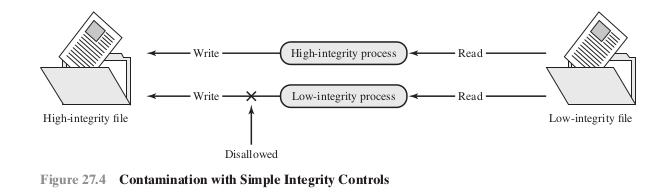
\includegraphics[width=10cm, keepaspectratio]{Bistarelli/img/cap_27/figura27.4.png}
\end{figure}

\subsection{Modello di integrità Clark-Wilson}
Un modello di integrità più elaborato e forse più pratico è stato proposto da Clark e Wilson. Il modello di integrità Clark-Wilson (CWM) è rivolto ad applicazioni commerciali piuttosto che militari e modella da vicino le reali operazioni commerciali. Il modello si basa su due concetti che sono tradizionalmente usati per applicare politiche di sicurezza commerciali:
\begin{itemize}
    \item \textbf{Transazioni ben formate:} Un utente non dovrebbe manipolare i dati arbitrariamente, ma solo in modi limitati che preservano o assicurano l'integrità dei dati.
    
    \item \textbf{Separazione dei compiti tra gli utenti:} Ogni persona autorizzata a creare o certificare una transazione ben formata non può essere autorizzata ad eseguirla (almeno contro dati di produzione). Il modello impone controlli di integrità sui dati e sulle transazioni che manipolano i dati.
\end{itemize}
I componenti principali del modello sono i seguenti:
\begin{itemize}
    \item \textbf{Elementi di dati vincolati (CDI):} Soggetti a severi controlli di integrità
    
    \item \textbf{Elementi di dati non vincolati (UDI):} Elementi di dati non controllati. Un esempio è un semplice file di testo
    
    \item \textbf{Procedure di verifica dell'integrità (IVP):} Destinate ad assicurare che tutte le CDI sono conformi a qualche modello di integrità e coerenza specifico dell'applicazione
    
    \item \textbf{Procedure di trasformazione (TP):} Transazioni di sistema che cambiano l'insieme delle CDI da uno stato coerente ad un altro Il CWM fa rispettare l'integrità per mezzo di regole di certificazione e applicazione sui TP. Le regole di certificazione sono restrizioni di politica di sicurezza sul comportamento di IVP e dei TP. 
    
Le regole di applicazione sono meccanismi di sicurezza integrati nel sistema che raggiungono gli obiettivi delle regole di certificazione.
\end{itemize}

\newpage
Le regole sono le seguenti:
\begin{center}
    \textbf{Cl:} Tutti gli IVP devono garantire adeguatamente che tutti i CDI siano in uno stato valido nel momento in cui l'IVP viene eseguito.
    
    \singlespacing

    \textbf{C2:} Tutti i TP devono essere certificati per essere validi. Cioè, devono portare un CDI ad uno stato finale valido, dato che è in uno stato valido per cominciare. Per ogni TP,  ogni insieme di CDI che può manipolare, il responsabile della sicurezza deve specificare una relazione che definisce tale esecuzione. Una relazione è quindi della forma (TPi, (CDIa, CDIb, CDIc . . . )), dove la lista dei CDI definisce un particolare insieme di argomenti per i quali il TP è stato certificato.
    
    \singlespacing

    \textbf{El:} Il sistema deve mantenere la lista di relazioni specificata nella regola C2 e deve assicurare che l'unica manipolazione di qualsiasi CDI sia da parte di un TP, dove il TP sta operando sul CDI come specificato in qualche relazione.
    
    \singlespacing

    \textbf{E2:} Il sistema deve mantenere una lista di relazioni della forma (UserID, TPi,(CDIa, CDIb, CDIc, . . . )), che mette in relazione un utente, un TP e gli oggetti dati che il TP può referenziare per conto di quell'utente. Deve assicurare che solo esecuzioni descritte in una delle relazioni.
    
    \singlespacing

    \textbf{C3:} L'elenco delle relazioni in E2 deve essere certificato per soddisfare il requisito di separazione dei compiti.
    
    \singlespacing
    
    \textbf{E3:} Il sistema deve autenticare l'identità di ogni utente che tenta di eseguire un TP.
    
    \singlespacing
    
    \textbf{C4:} Tutti i TP devono essere certificati per scrivere in un CDI di sola appendice (il log) tutte le informazioni necessarie per permettere di ricostruire la natura dell'operazione.
    
    \singlespacing
    
    \textbf{C5:} Ogni TP che prende un UDI come valore di ingresso deve essere certificato per eseguire solo trasformazioni valide, oppure nessuna trasformazione, per ogni possibile valore dell'UDI. La trasformazione dovrebbe prendere l'input da un UDI, o l'UDI viene rifiutata. Tipicamente, questo è un programma di modifica.
    
    \singlespacing
    
    \textbf{E4:} Solo l'agente autorizzato a certificare entità può cambiare la lista di tali entità associate ad altre entità: in particolare, la lista dei TP  associati con un CDI e la lista degli utenti associati a un TP. Un agente che può certificare un'entità non può avere alcun diritto di esecuzione rispetto a tale entità.
\end{center}

\begin{figure}[H]
	\centering
    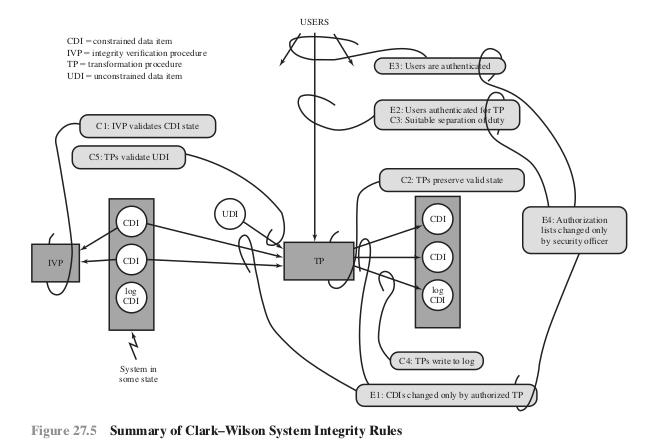
\includegraphics[width=10cm, keepaspectratio]{Bistarelli/img/cap_27/figura27.5.png}
\end{figure}

\newpage
\subsection{Modello Muraglia Cinese}
Il Chinese Wall Model (CWM) ha un approccio abbastanza diverso per specificare integrità e riservatezza rispetto a qualsiasi approccio che abbiamo esaminato finora. Il modello è stato sviluppato per applicazioni commerciali in cui possono sorgere conflitti di interesse. Il modello fa uso di concetti di accesso sia discrezionali che obbligatori. L'idea principale dietro il CWM è un concetto che è comune nelle professioni legali, che è quello di usare una cosiddetta muraglia cinese per prevenire un conflitto di interessi. Un esempio dal mondo finanziario è quello di un analista di mercato che lavora per un'istituzione finanziaria che fornisce servizi aziendali. Un analista non può essere autorizzato a fornire consigli a una società quando l'analista ha informazioni riservate (conoscenza privilegiata) sui piani o lo stato di un concorrente. Tuttavia l'analista è libero di consigliare più società che non sono in concorrenza tra loro e di attingere alle informazioni di mercato che sono aperte al pubblico. 

\singlespacing

Gli elementi del modello sono i seguenti:

\begin{itemize}
    \item \textbf{Soggetti:} Entità attive che potrebbero voler accedere a oggetti protetti. include utenti e processi

    \item \textbf{Informazioni:} Informazioni aziendali organizzate in una gerarchia con tre livelli
    
    \begin{itemize}
        \item \textbf{Oggetti:} Singoli elementi di informazione, ciascuno riguardante una singola società
        
        \item \textbf{Set di dati (DS):} Tutti gli oggetti che riguardano la stessa società
        
        \item \textbf{Classe di conflitto di interessi (CI):} Tutti i set di dati le cui società sono in concorrenza

    \end{itemize}
    \item \textbf{Regole di accesso:} Regole per l'accesso in lettura e scrittura
\end{itemize}

A differenza dei modelli che abbiamo studiato finora, il CWM non assegna livelli di sicurezza a soggetti e oggetti e quindi non è un vero modello sicuro multi-livello. Invece, la storia del precedente accesso di un soggetto determina il controllo dell'accesso. La base della politica della muraglia cinese è che i soggetti possono accedere solo alle informazioni che non è ritenuto in conflitto con qualsiasi altra informazione che già possiedono. Una volta che un soggetto accede alle informazioni di un set di dati, una muraglia è impostata per proteggere le informazioni in altri insiemi di dati nello stesso CI. Il soggetto può accedere alle informazioni su un lato del del muro ma non dall'altro lato. Inoltre, le informazioni in altri CI non sono inizialmente Inoltre, le informazioni in altri IC non sono inizialmente considerate su un lato o l'altro del muro, ma all'aperto. Quando lo stesso soggetto effettua ulteriori accessi in altri IC, la forma del muro cambia per mantenere la protezione desiderata. Inoltre, ogni soggetto è controllato dal proprio pareti per i diversi soggetti che sono diverse.

\singlespacing

Per far rispettare la politica della muraglia cinese, sono necessarie due regole. Per indicare la similarità con le due regole BLP, gli autori hanno dato loro gli stessi nomi.

\singlespacing

\begin{center}
    La prima regola è la \textbf{semplice regola di sicurezza}
\end{center}

Regola di sicurezza semplice:
\begin{itemize}
    \item O si trova nello stesso DS di un oggetto a cui S ha già avuto accesso
    \item O appartiene a un CI da cui S non ha ancora avuto accesso a nessuna informazione.
\end{itemize}

\begin{figure}[H]
	\centering
    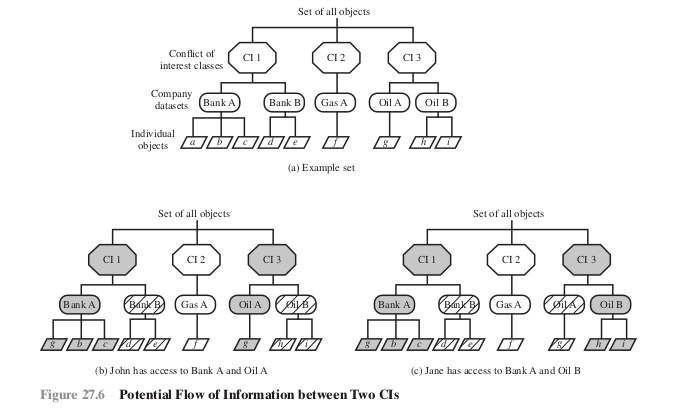
\includegraphics[width=10cm, keepaspectratio]{Bistarelli/img/cap_27/figura27.6.png}
\end{figure}

John ha fatto la sua prima richiesta di lettura a qualsiasi oggetto in questo set per un oggetto nella Banca A DS. Poiché John non ha precedentemente avuto accesso ad un oggetto in nessun altro DS in CI 1, l'accesso accesso è concesso. Inoltre, il sistema deve ricordare che l'accesso è stato concesso in modo che ogni successiva richiesta di accesso a un oggetto nella Banca B DS sarà negata. Qualsiasi richiesta di accesso ad altri oggetti nella Banca A DS è concessa. In un momento successivo, John richiede l'accesso ad un oggetto nella Banca A DS. Poiché non c'è conflitto, questo accesso viene concesso, ma viene creato un muro che proibisce il successivo accesso all'Oil B DS, come mostrato nella Figura 27.6b. Allo stesso modo, la Figura 27.6c riflette la storia di accesso alternativo di Jane. Nel nostro esempio, John ha accesso a Oil A DS e Bank A DS; Jane ha accesso a Oil B DS e Bank A DS. Se John è autorizzato a leggere dall'Oil A DS e scrivere nel Bank A DS, John può trasferire informazioni sull'olio A nel Bank A DS; ciò è indicato dal cambiamento del valore del primo oggetto sotto il Bank A DS a g. I dati possono poi essere letti da Jane. Così, Jane avrebbe accesso alle informazioni sia sul petrolio A che sul petrolio B, creando un conflitto di interessi.

\begin{center}
    Per prevenire questo, il CWM ha una \textbf{seconda regola}
\end{center}

Regola della proprietà: Un soggetto S può scrivere un oggetto O solo se:

\begin{itemize}
    \item S può leggere O secondo la regola di sicurezza semplice, E
    
    \item Tutti gli oggetti che S può leggere sono nella stessa DS di O.
\end{itemize}

Detto altrimenti, o il soggetto non può scrivere affatto, o l'accesso di un soggetto (sia lettura e scrittura) è limitato ad un singolo set di dati. Così, nella figura 27.6, né John né Jane ha accesso in scrittura a qualsiasi oggetto nell'universo complessivo dei dati.

\singlespacing

La regola proprietà è abbastanza restrittiva. Tuttavia, in molti casi, un utente ha solo ha bisogno dell'accesso in lettura perché l'utente sta eseguendo qualche ruolo di analisi.

\singlespacing

Per facilitare in qualche modo la restrizione di scrittura, il modello include il concetto di dati sanificati. In sostanza, i dati sanificati sono dati che possono essere derivati dai dati aziendali ma che non possono essere usati per scoprire l'identità della società. Qualsiasi DS che consiste esclusivamente di dati sanificati non ha bisogno di essere protetto da un muro; quindi, le due regole CWM non si non si applicano a tali DS.

\newpage
\section{Il concetto di sitemi fidati}
\subsection{Applicazione sicurezza multilivello}
\paragraph{Sicurezza multilivello (MLS)} è un modo di funzionamento del sistema in cui:

\begin{itemize}
    \item \textbf{Due o più livelli di sicurezza} delle informazioni possono essere gestiti simultaneamente all'interno dello stesso sistema quando alcuni utenti che hanno accesso al sistema non hanno né un nulla osta di sicurezza né la necessità di sapere per alcuni dei dati gestiti dal sistema.
    
    \item \textbf{La separazione degli utenti e del materiale classificato sulla base} dell'autorizzazione e del livello di classificazione dipendono dal controllo del sistema operativo.

\end{itemize}
La sicurezza multilivello è interessante quando c'è la necessità di mantenere una risorsa, come un file system o un database in cui sono definiti più livelli di sensibilità dei dati. La gerarchia potrebbe essere semplice come due livelli (ad esempio, pubblico e proprietario) o potrebbe avere molti livelli (ad esempio, il militare non classificato, riservato, confidenziale, segreto, top secret). Le tre sezioni precedenti ci hanno introdotto agli elementi essenziali della sicurezza multilivello. 

\singlespacing

In questa sezione, esaminiamo due applicazioni in cui sono stati applicati i concetti di MLS: 

\begin{enumerate}
    \item Sistema di controllo degli accessi basato sui ruoli.
    
    \item La sicurezza dei database.
\end{enumerate}
\newpage
\subsection{Sicurezza multilivello per il controllo dell'accesso basato sui ruoli}

Mostra come un sistema di controllo degli accessi basato su regole (RBAC) può essere usato per implementare le regole di sicurezza multilivello BLP. Ricordiamo che la specifica ANSI standard RBAC ANSI includeva il concetto di funzioni amministrative, che forniscono la capacità di creare, cancellare e mantenere elementi e relazioni RBAC. È utile quindi assegnare ruoli amministrativi speciali a queste funzioni. Con questo in mente, La Tabella 27.2 riassume i componenti di un RBAC.

\singlespacing

La seguente specifica formale indica come un sistema RBAC può essere usato per implementare l'accesso MLS:

\begin{itemize}
    \item \textbf{Vincolo sugli utenti:}

    Per ogni utente u nell'insieme degli utenti U, viene assegnato un nulla osta di sicurezza L(u). Formalmente, qualsiasi u $\in$ U $[L(u) è dato]$.
    
    \item \textbf{Vincoli sui permessi:}

    Ogni permesso assegna un permesso di lettura o scrittura a un oggetto o, e ogni oggetto ha un permesso di lettura e uno di scrittura. Tutti gli oggetti hanno una classificazione di sicurezza. Formalmente, $P = \{(o,r),(o,w)$ o è un oggetto nel sistema\} qualsiasi o $\in$ P[L(o) è dato].
    
    \item \textbf{Definizioni:}
    
    Il livello di lettura di un ruolo r, denotato r-level(r), è il minimo limite superiore dei livelli di sicurezza degli oggetti per i quali (o, r) è nelle autorizzazioni di r. Il livello w di un ruolo r (denotato w-level(r)) è il massimo limite inferiore (glb) dei livelli di sicurezza degli oggetti o per i quali (o, w) è nelle permessi di r, se tale glb esiste. Se il glb non esiste, il livello w è indefinito.
    
    \item \textbf{Vincoli su UA:}
    
    Ogni ruolo r ha un livello di scrittura definito, denotato w-level(r). Per ogni assegnazione dell'utente, l'autorizzazione dell'utente deve dominare il livello r del ruolo ed essere dominata dal livello w del ruolo. Formalmente, qualsiasi r $\in$ UA [w-level(r) è definito]; qualsiasi (u,r) $\in$ UA [L(u) $>=$ r-livello(r)]; qualsiasi (u,r) $\in$ UA [L(u) $<=$ w-livello(r)].
    

\end{itemize}

Le definizioni e i vincoli precedenti applicano il modello BLP. Un ruolo può includere permessi di accesso per più oggetti. Il livello r del ruolo indica la più alta classificazione di sicurezza per gli oggetti assegnati al ruolo. Così, la semplice proprietà di sicurezza (nessuna lettura) richiede che un utente possa essere assegnato a un ruolo solo se l'autorizzazione dell'utente è almeno pari al livello r del ruolo. Allo stesso modo, il livello w del ruolo indica la classificazione di sicurezza più bassa dei suoi oggetti. La proprietà sicurezza (no write down) richiede che un utente sia assegnato a un ruolo solo se il suo non è superiore al livello w del ruolo.

\begin{figure}[H]
	\centering
    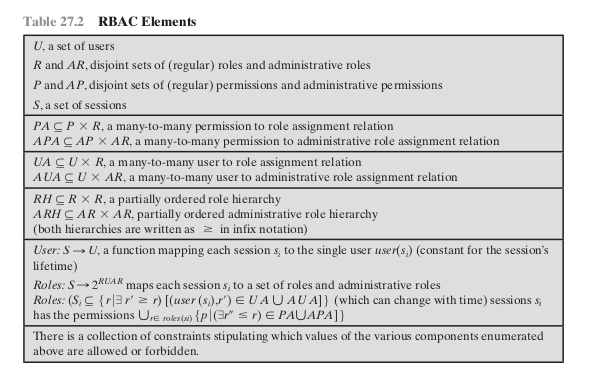
\includegraphics[width=10cm, keepaspectratio]{Bistarelli/img/cap_27/tabella27.2.png}
\end{figure}


\subsection{Sicurezza dei database e sicurezza multilivello}

L'aggiunta della sicurezza multilivello a un sistema di database aumenta la complessità della funzione di controllo dell'accesso e del design del database stesso. Una questione chiave è la granularità della classificazione. I seguenti sono possibili metodi per imporre la sicurezza multilivello su un database relazionale, in termini di granularità di classificazione (vedi Figura 27.9):
\begin{itemize}
    \item \textbf{Intero database:} Questo semplice approccio è facilmente realizzabile su una piattaforma MLS. Un intero database, come un database finanziario o personale, potrebbe essere classificato come confidenziale o riservato e mantenuto su un server con altri file.
    
    \item \textbf{Tabelle individuali (relazioni):} Per alcune applicazioni, è appropriato assegnare classificazione a livello di tabella. Nell'esempio della Figura 27.9a, sono definiti due livelli di classificazione:
    \begin{itemize}
        \item Unrestricted (U)
        \item Restricted (R)
    \end{itemize}
\end{itemize}

La tabella Employee contiene informazioni sensibili sullo stipendio ed è classificata ristretta, mentre la tabella tabella Department è illimitata. Questo livello di granularità è relativamente facile da implementare e applicare.

\begin{itemize}
    \item \textbf{Colonne individuali (attributi):} Un amministratore della sicurezza può scegliere di determinare la classificazione sulla base degli attributi, in modo che le colonne selezionate sono classificate. Nell'esempio della Figura 27.9b, l'amministratore determina che le informazioni sullo stipendio e l'identità dei responsabili di reparto sono informazioni riservate.
    
    \item \textbf{Righe individuali (tuple):} altre circostanze, può avere senso assegnare livelli di classificazione sulla base di singole righe che corrispondono a certe proprietà. Nell'esempio della figura 27.9c, tutte le righe della tabella Department che contengono informazioni relative al dipartimento di contabilità (Dept. ID = 4), e tutte le righe nella tabella Employee per le quali lo stipendio è maggiore di 50K sono limitate.
    
    \item \textbf{Elementi individuali:} Lo schema più difficile da implementare e gestire è uno in cui i singoli elementi possono essere classificati selettivamente. Nell'esame Figura 27.9d, le informazioni sullo stipendio e l'identità del manager del eparto contabilità sono limitate
\end{itemize}

La granularità dello schema di classificazione influisce sul modo in cui il controllo dell'accesso viene applicato. In particolare, gli sforzi per prevenire l'inferenza dipendono dalla granularità della classificazione.

\begin{figure}[H]
	\centering
    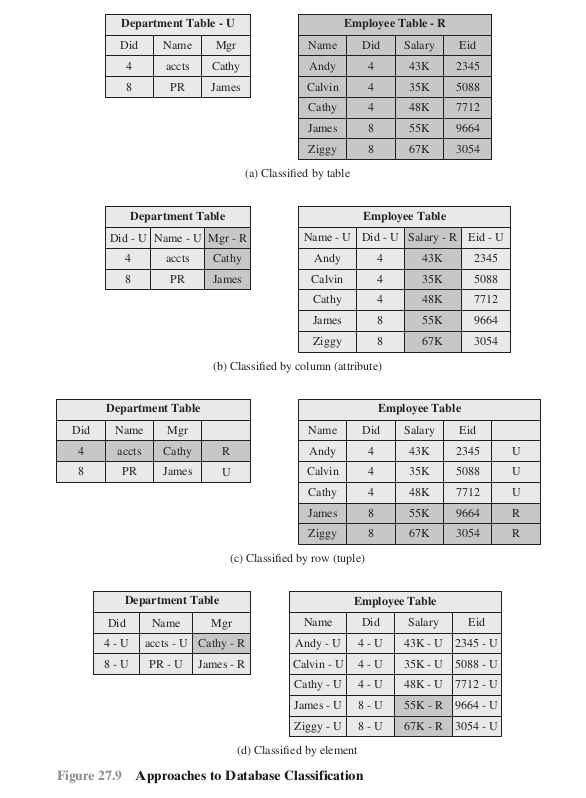
\includegraphics[width=10cm, keepaspectratio]{Bistarelli/img/cap_27/figura27.9.png}
\end{figure}


\section{Trusted Computing e il Trusted Platform Module}

Il trusted platform module (TPM) è un concetto standardizzato da un consorzio industriale consorzio industriale, il Trusted Computing Group. Il TPM è un modulo hardware che è al il cuore di un approccio hardware/software all'informatica di fiducia. Infatti, il termine trusted computing (TC) è ora usato nell'industria per riferirsi a questo tipo di approccio hardware/approccio hardware/software. L'approccio TC impiega un chip TPM nella scheda madre del personal computer o una smart card o integrato nel processore principale, insieme all'hardware e al software che in qualche modo è stato approvato o certificato per lavorare con il TPM.

\singlespacing

Il TPM genera chiavi che condivide con i componenti vulnerabili che passano dati all'interno del sistema, come i dispositivi di archiviazione, i componenti di memoria e l'hardware audio/visivo. hardware audio/video. Le chiavi possono essere usate per crittografare i dati che fluiscono attraverso la macchina. Il TPM funziona anche con il software abilitato a TC, incluso il sistema operativo e le applicazioni.

\singlespacing

Il software può essere sicuro che i dati che riceve sono affidabili, e il sistema può essere sicuro che il software stesso sia affidabile.

\singlespacing

Per ottenere queste caratteristiche, TC fornisce tre servizi di base: avvio autenticato, certificazione e crittografia.

\newpage
\subsection{Servizio di avvio autenticato}

Il servizio di avvio autenticato è responsabile dell'avvio dell'intero sistema operativo in fasi e assicurando che ogni porzione del sistema operativo, quando viene caricata, sia una versione che è approvato per l'uso. Tipicamente, l'avvio di un sistema operativo inizia con un piccolo pezzo di codice nella ROM. Questo pezzo porta altro codice dal blocco di avvio sul disco rigido e trasferisce l'esecuzione a quel codice. Questo processo continua con blocchi sempre più grandi del codice del sistema operativo fino a quando l'intera procedura di avvio del sistema operativo è completa e il sistema operativo residente è avviato. Ad ogni stadio, l'hardware del TC controlla che il software valido sia stato portato dentro. Questo può essere fatto verificando una firma digitale associata al software.

\singlespacing

Il TPM tiene un registro a prova di manomissione del processo di caricamento, usando una funzione di hash crittografica per rilevare qualsiasi manomissione del registro. Quando il processo è completato, il registro a prova di manomissione contiene un record che stabilisce esattamente quale versione del sistema operativo e i suoi vari moduli sono in esecuzione. È ora possibile espandere il confine di fiducia per includere ulteriore hardware e applicazioni e software di utilità. Il sistema abilitato TC mantiene una lista approvata di componenti hardware e software approvati. Per configurare un pezzo di hardware o caricare un software, il sistema controlla se il componente è nella lista approvata, se è firmato digitalmente (dove applicabile), e se il suo numero di serie non è stato revocato. Il risultato è una configurazione di hardware, software di sistema e applicazioni che è in uno stato ben definito con componenti approvati.

\subsection{Servizio di certificazione}

Una volta che una configurazione è raggiunta e registrata dal TPM, il TPM può certificare la configurazione ad altre parti. Il TPM può produrre un certificato digitale firmando una descrizione formattata delle informazioni di configurazione usando la chiave privata del TPM. Così, un altro utente, sia un utente locale che un sistema remoto, può avere fiducia che una configurazione inalterata è in uso perché:

\begin{enumerate}
    \item Il TPM è considerato affidabile. Non abbiamo bisogno di un'ulteriore certificazione del TPM stesso.
    
    \item Solo il TPM possiede la chiave privata di questo TPM. Un destinatario della configurazione può usare la chiave pubblica del TPM per verificare la firma (vedi Figura 2.7b).
\end{enumerate}
Per assicurare che la configurazione sia puntuale, un richiedente emette una "sfida" sotto forma di un numero casuale quando richiede un certificato firmato dal TPM.

\singlespacing

Il TPM firma un blocco di dati che consiste nelle informazioni di configurazione con il numero casuale aggiunto ad esso. Il richiedente può quindi verificare che il certificato sia valido e aggiornato.

\singlespacing

Lo schema TC prevede un approccio gerarchico alla certificazione. Il TPM certifica la configurazione hardware/OS. Poi il sistema operativo può certificare la presenza e la configurazione dei programmi applicativi. Se un utente si fida del TPM e si fida della versione certificata del sistema operativo, allora l'utente può avere fiducia nella configurazione dell'applicazione.

\subsection{Servizio di crittografia}
Il servizio di crittografia permette la crittografia dei dati in modo tale che i dati possano essere decifrati solo da una certa macchina, e solo se questa macchina è in una certa configurazione. Ci sono diversi aspetti di questo servizio.

\singlespacing

In primo luogo, il TPM mantiene una chiave segreta principale unica per questa macchina. Da questa chiave, il TPM genera una chiave di crittografia segreta per ogni possibile configurazione di quella macchina. Se i dati sono criptati mentre la macchina è in una configurazione, i dati possono essere decifrati solo usando quella stessa configurazione. Se una configurazione diversa viene creata sulla macchina, la nuova configurazione non sarà in grado di decifrare i dati crittografati da una configurazione diversa.

\singlespacing

Questo schema può essere esteso verso l'alto, come si fa con la certificazione. Così, è possibile fornire una chiave di crittografia ad un'applicazione in modo che l'applicazione possa criptare i dati, e la decriptazione possa essere fatta solo dalla versione desiderata dell'applicazione desiderata che gira sulla versione desiderata del sistema operativo desiderato. Questi dati crittografati possono essere memorizzati localmente, recuperabili solo dall'applicazione che li ha memorizzati, o trasmessi a un'applicazione peer su una macchina remota. L'applicazione peer dovrebbe essere nella stessa configurazione per decifrare i dati.

\newpage
\subsection{Funzioni TPM}
Per dare un'idea del funzionamento di un sistema TC/TPM, guardiamo la funzione di memorizzazione protetta. Il TPM genera e memorizza un certo numero di chiavi crittografia in una gerarchia di fiducia. Alla radice della gerarchia c'è una chiave radice di memorizzazione generata dal TPM e accessibile solo per l'uso del TPM. Da questa chiave, altre chiavi possono essere generate e protette dalla crittografia con chiavi più vicine alla radice della gerarchia.

Una caratteristica importante delle Trusted Platforms è che un oggetto protetto dal TPM può essere "sigillato" ad un particolare stato del software in una piattaforma. Quando l'oggetto protetto TPM viene creato, il creatore indica lo stato del software che deve esistere se il segreto deve essere rivelato. Quando un TPM scarta l'oggetto protetto TPM (all'interno del TPM e nascosto alla vista), il TPM controlla che lo stato attuale del software corrisponda allo stato del software indicato. Se corrispondono, il TPM permette l'accesso al segreto. Se non non corrispondono, il TPM nega l'accesso al segreto.

\singlespacing

La figura 27.12 fornisce un esempio di questa protezione. In questo caso, c'è un file criptato sulla memoria locale a cui un'applicazione utente desidera accedere. I seguenti passi da compiere:

\begin{enumerate}
    \item La chiave simmetrica che è stata usata per criptare il file è memorizzata con il file. La chiave stessa è criptata con un'altra chiave a cui il TPM ha accesso. La chiave protetta è presentata al TPM con una richiesta di rivelare la chiave all'applicazione.
    
    \item Associata alla chiave protetta è una specifica della configurazione hardware/software che può avere accesso alla chiave. Il TPM verifica che la configurazione corrente corrisponda alla configurazione richiesta per rivelare la chiave. Inoltre, l'applicazione richiedente deve essere specificamente autorizzata ad accedere alla chiave. Il TPM usa un protocollo di autorizzazione per verificare l'autorizzazione.
    
    \item Se la configurazione corrente permette l'accesso alla chiave protetta, allora il TPM decifra la chiave e la passa all'applicazione.
    
    \item L'applicazione usa la chiave per decifrare il file. L'applicazione è affidabile per poi scartare la chiave in modo sicuro.
\end{enumerate}
La crittografia di un file procede in modo analogo. In quest'ultimo caso, un processo richiede una chiave simmetrica per cifrare il file. Il TPM fornisce quindi una versione criptata della chiave da memorizzare con il file.

\begin{figure}[H]
	\centering
    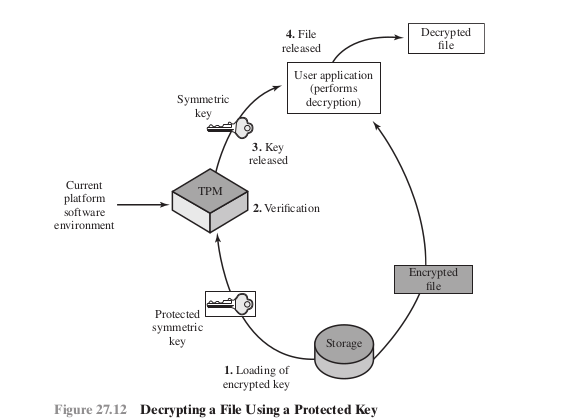
\includegraphics[width=10cm, keepaspectratio]{Bistarelli/img/cap_27/figura27.12.png}
\end{figure}

\newpage
\subsection{Requisiti}
Il CC definisce un insieme comune di potenziali requisiti di sicurezza da usare nella valutazione. Il termine obiettivo della valutazione (TOE) si riferisce a quella parte del prodotto o sistema che è soggetto alla valutazione. I requisiti rientrano in due categorie:
\begin{enumerate}
    \item \textbf{Requisiti funzionali}
    
    Definiscono il comportamento di sicurezza desiderato. I documenti CC stabiliscono un insieme di componenti funzionali di sicurezza che forniscono un modo standard di esprimere i requisiti funzionali di sicurezza per un TOE.
    
    \item \textbf{Requisiti di sicurezza}
    
    La base per ottenere la fiducia che le misure di sicurezza dichiarate misure di sicurezza dichiarate siano efficaci e implementate correttamente. I documenti CC stabiliscono un insieme di componenti di garanzia che forniscono un modo standard di esprimere i requisiti di garanzia per un TOE.
\end{enumerate}

Sia i requisiti funzionali che quelli di garanzia sono organizzati in classi:

\begin{center}
    \textbf{Una classe è una collezione di requisiti che condividono un obiettivo o un intento comune.}
\end{center}

Le tabelle 27.3 e 27.4 definiscono brevemente le classi per i requisiti funzionali e di garanzia. Ciascuna di queste classi contiene un certo numero di famiglie. I requisiti all'interno di ogni famiglia condividono obiettivi di sicurezza, ma differiscono per enfasi o rigore. Per esempio, la classe di audit contiene sei famiglie che si occupano di vari aspetti dell'auditing (ad es, generazione di dati di audit, analisi di audit e memorizzazione di eventi di audit). Ogni famiglia, a sua volta, contiene uno o più componenti. Un componente descrive un insieme specifico di requisiti di sicurezza requisiti di sicurezza ed è il più piccolo insieme selezionabile di requisiti di sicurezza da includere nelle strutture definite nel CC.

\begin{figure}[H]
	\centering
    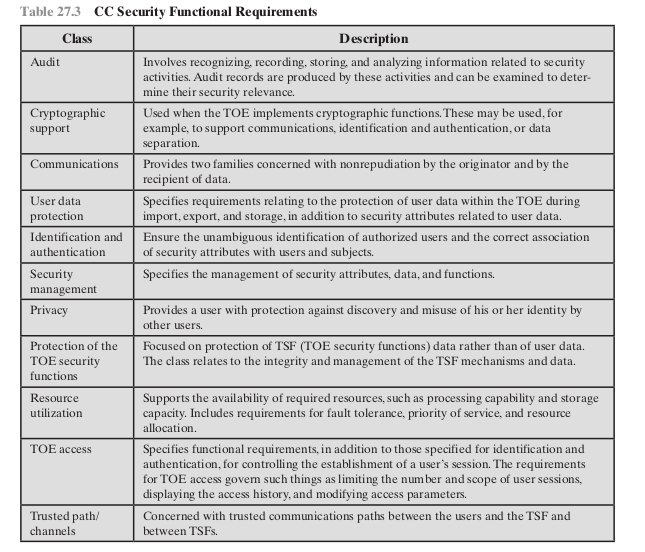
\includegraphics[width=10cm, keepaspectratio]{Bistarelli/img/cap_27/tabella27.3.png}
\end{figure}

\begin{figure}[H]
	\centering
    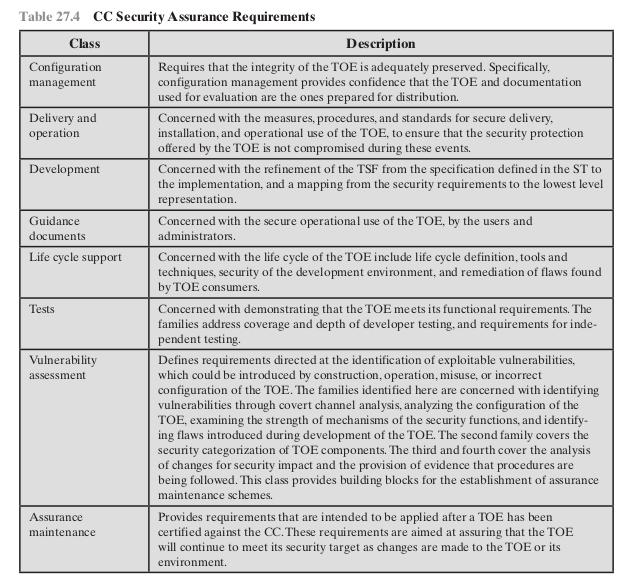
\includegraphics[width=10cm, keepaspectratio]{Bistarelli/img/cap_27/tabella27.4.png}
\end{figure}
\newpage
\subsection{Profili e Obiettivi}
Il CC definisce anche due tipi di documenti che possono essere generati usando i requisiti definiti dal CC.

\begin{itemize}
    \item \textbf{Profili di protezione (PP):} Definiscono un insieme indipendente dall'implementazionedi requisiti e obiettivi di sicurezza per una categoria di prodotti o sistemi che soddisfano esigenze simili dei consumatori per la sicurezza informatica.
    
    Un PP è inteso essere riutilizzabile e definire requisiti che sono noti per essere utili ed efficaci nel soddisfare gli obiettivi identificati. Il concetto di PP è stato sviluppato per supportare la definizione di standard funzionali e come aiuto alla formulazione di specifiche di approvvigionamento. Il PP riflette la sicurezza dell'utente esigenze degli utenti.
    
    \item \textbf{Obiettivi di sicuressa(ST):} Contengono gli obiettivi e i requisiti di sicurezza IT di uno specifico TOE identificato e definisce le misure funzionali e di garanzia offerte da quel TOE per soddisfare i requisiti dichiarati. 
\end{itemize}
\newpage
\subsection{Esempio di protezione di un profilo}
Il profilo di protezione per una smart card, sviluppato dallo Smart Card Security User Group, fornisce un semplice esempio di PP.

\singlespacing

Questo PP descrive i requisiti di sicurezza IT per una smart card da usare in connessione con applicazioni sensibili, come i sistemi di pagamento finanziario dell'industria bancaria. Il livello di garanzia per questo PP è EAL 4, che è descritto nella seguente sottosezione. Il PP elenca le minacce che devono essere affrontate da un prodotto che dichiara di essere conforme a questo PP. Le minacce includono seguenti:
\begin{itemize}
    \item \textbf{Sondaggio fisico:} Può comportare la lettura di dati dal TOE attraverso tecniche comunemente impiegate nell'analisi dei guasti IC e negli sforzi di reverse engineering IC.
    
    \item \textbf{Input non valido:} L'input non valido può assumere la forma di operazioni che non sono correttamente, richieste di informazioni oltre i limiti del registro, o tentativi di trovare ed eseguire comandi non documentati. Il risultato di un tale attacco può essere una compromissione delle funzioni di sicurezza, la generazione di errori sfruttabili nel funzionamento, o il rilascio di dati protetti.
    
    \item \textbf{Collegamento di più operazioni:} Un attaccante può osservare usi multipli di risorse o servizi e, collegando queste osservazioni, dedurre informazioni che possono rivelare dati sulla funzione di sicurezza.

\end{itemize}

Dopo un elenco di minacce, il PP passa alla descrizione degli obiettivi di sicurezza. Questi riflettono l'intento dichiarato di contrastare le minacce identificate e/o conformarsi a qualsiasi politiche di sicurezza organizzativa identificate. Sono elencati diciannove obiettivi, tra cui i seguenti:

\begin{itemize}
    \item \textbf{Audit:} Il sistema deve fornire i mezzi per registrare determinati eventi rilevanti per la sicurezza eventi rilevanti per la sicurezza, in modo da assistere un amministratore nell'individuazione potenziali attacchi o configurazioni errate delle caratteristiche di sicurezza del sistema che lo lascerebbero suscettibile di attacco.
    
    \item \textbf{Inserimento dei guasti:} Il sistema deve essere resistente a sondaggi ripetuti attraverso inserimento di dati errati.
    
    \item \textbf{Perdita di informazioni:} Il sistema deve fornire i mezzi per controllare e limitare la perdita di informazioni nel sistema in modo che nessuna informazione utile sia rivelata attraverso le linee di alimentazione, terra, clock, reset o I/O.
    
\end{itemize}

I requisiti di sicurezza sono forniti per contrastare minacce specifiche e per supportare politiche specifiche sotto specifiche ipotesi. Il PP elenca requisiti specifici in tre aree generali: requisiti funzionali di sicurezza del TOE, requisiti di sicurezza del TOE, e requisiti di sicurezza per l'ambiente IT.

\singlespacing

Nell'area dei requisiti funzionali di sicurezza, il PP definisce 42 requisiti delle classi disponibili di requisiti funzionali di sicurezza (vedi tabella 27.3).

\singlespacing

Per esempio, per l'auditing di sicurezza, il PP stabilisce cosa deve controllare il sistema; quali informazioni devono essere registrate; quali sono le regole per monitorare, operare e proteggere i registri, e così via. I requisiti funzionali sono anche elencati da le altre classi di requisiti funzionali, con dettagli specifici per il funzionamento della smart card.

\singlespacing

Il PP definisce 24 requisiti di garanzia della sicurezza dalle classi disponibili di requisiti di garanzia della sicurezza (vedi tabella 27.4). Questi requisiti sono stati scelti per dimostrare:

\begin{itemize}
    \item La qualità della progettazione e della configurazione del prodotto
    
    \item Che viene fornita una protezione adeguata durante la progettazione e l'implementazione del prodotto
    
    \item  Che il test del prodotto da parte del fornitore rispetta parametri specifici
    
    \item Che la funzionalità di sicurezza non è compromessa durante la consegna del prodotto
    
    \item che la guida per l'utente, compresi i manuali del prodotto relativi all'installazione, alla manutenzione e all'uso, siano di una qualità specifica, la manutenzione e l'uso, siano di una specifica qualità e adeguatezza
\end{itemize}
Il PP elenca anche i requisiti di sicurezza dell'ambiente IT. Questi coprono i seguenti argomenti:

\begin{itemize}
    \item Distribuzione delle chiavi crittografiche
    
    \item Distruzione della chiave crittografica
    
    \item Ruoli di sicurezza
\end{itemize}

\newpage
\section{Assicurazione e valutazione}
La garanzia può essere definita come una misura di fiducia che le caratteristiche di sicurezza e l'architettura di un sistema informativo (IS) mediano e applicano accuratamente la politica di sicurezza. Se si fa affidamento sulle caratteristiche di sicurezza di un IS per proteggere informazioni classificate o sensibili e limitare l'accesso degli utenti, le caratteristiche devono essere testate per assicurare che la politica di sicurezza sia applicata. Come per qualsiasi altro aspetto della sicurezza informatica, le risorse dedicate alla garanzia devono essere sottoposte a una sorta di analisi costi-benefici per determinare quale quantità di sforzo sia ragionevole per il livello di garanzia desiderato.

\subsection{Destinatari}
Il design delle misure di garanzia dipende in parte dal pubblico a cui queste misure. Cioè, nello sviluppare un grado di fiducia nelle misure di sicurezza, dobbiamo specificare quali individui o gruppi possiedono quel grado di fiducia. Il documento del CC sull'assicurazione elenca i seguenti destinatari:

\begin{itemize}
    \item \textbf{Consumatori:} Selezionano le caratteristiche e le funzioni di sicurezza per un sistema e determinano i livelli richiesti di garanzia di sicurezza.
    
    \item \textbf{Sviluppatori:} Rispondono ai requisiti di sicurezza reali o percepiti dai consumatori; interpretare le dichiarazioni dei requisiti di sicurezza e determinare gli approcci e livello di sforzo.
    
    \item \textbf{Valutatori:} Usano i requisiti di garanzia come una dichiarazione obbligatoria di criteri di valutazione quando valutano le caratteristiche e i controlli di sicurezza.
\end{itemize}

I valutatori possono essere nella stessa organizzazione dei consumatori o un team di valutazione di terze parti.

\newpage
\subsection{Ambito di garanzia}

La garanzia si occupa delle caratteristiche di sicurezza dei prodotti IT, come computer, database, sistemi operativi e sistemi completi. La garanzia si applica a i seguenti aspetti di un sistema:
\begin{itemize}
    \item \textbf{Requisiti:} Questa categoria si riferisce ai requisiti di sicurezza di un prodotto

    \item \textbf{Politica di sicurezza:} Sulla base dei requisiti, può essere definita una politica di sicurezza

    \item \textbf{Progettazione del prodotto:} Sulla base dei requisiti e della politica di sicurezza

    \item \textbf{Implementazione del prodotto:} Basato sulla progettazione

    \item \textbf{Funzionamento del sistema:} Include l'uso ordinario più la manutenzione
\end{itemize}

In ogni area, si possono adottare diversi approcci per fornire garanzie. 

\singlespacing

I possibili approcci:

\begin{itemize}
    \item Analisi e controllo dei processi e delle procedure
    
    \item Verifica dell'applicazione dei processi e delle procedure

    \item Analisi della corrispondenza tra le rappresentazioni del progetto TOE
    
    \item Analisi della rappresentazione del progetto TOE rispetto ai requisiti
    
    \item Verifica delle prove
    
    \item Analisi dei documenti di guida
    
    \item Analisi dei test funzionali sviluppati e dei risultati forniti
    
    \item Test funzionali indipendenti
    
    \item Analisi delle vulnerabilità (inclusa l'ipotesi di difetti)
    
    \item Penetration Testing
\end{itemize}

Siccome viene fornita una visione un po' diversa degli elementi di garanzia. Questa relazione è basata sull'esperienza con le valutazioni di Orange Book, ma è rilevante per gli attuali sforzi di sviluppo di prodotti affidabili. 
L'autore vede la garanzia come comprendente i seguenti requisiti:

\begin{itemize}
    \item \textbf{Architettura del sistema} 
    
    Riguarda sia la fase di sviluppo del sistema che la fase operativa del sistema. Esempi di tecniche per aumentare il livello di garanzia durante la fase di sviluppo includono la progettazione modulare del software, la stratificazione e l'astrazione dei dati/nascondere le informazioni.
    
    \item\textbf{Integritò del sistema}
    
    Riguarda il corretto funzionamento dell'hardware e del firmware ed è tipicamente soddisfatto dall'uso periodico di software diagnostico.
    
    \item \textbf{Test del sistema}
    
    Assicura che le caratteristiche di sicurezza siano state testate a fondo. Questo include il test delle operazioni funzionali, il test dei requisiti di sicurezza, e test di possibili penetrazioni.
    
    \item \textbf{Specifica e verifica del design}
    
    Affronta la correttezza del design e dell'implementazione del sistema progettazione e implementazione del sistema rispetto alla politica di sicurezza del sistema. Idealmente, possono essere usati metodi formali di verifica.
    
    \item \textbf{Gestione fidata della struttura}
    
    Si occupa dell'amministrazione del sistema. Un approccio è quello di separare i ruoli di operatore del sistema e di amministratore della sicurezza. Un altro approccio è la specificazione dettagliata di politiche e procedure con meccanismi per la revisione.
    
    \item \textbf{Recupero affidabile}
    
    Fornisce il corretto funzionamento delle funzioni di sicurezza dopo che un sistema si riprende da guasti, crash o incidenti di sicurezza.
    
    \item \textbf{Distribuzione fidata}
    
    Assicura che hardware, firmware e software protetti non subiscano modifiche non autorizzate durante il transito dal fornitore al cliente
     
    \item \textbf{Gestione della configurazione}
     
    I requisiti sono inclusi per la configurazione controllo, audit, gestione e contabilità
\end{itemize}
Così, vediamo che la garanzia si occupa della progettazione, dell'implementazione e del funzionamento delle risorse protette e delle loro funzioni e procedure di sicurezza. È importante notare che la garanzia è un processo, non un risultato. Cioè, la garanzia deve essere un'attività attività continua, che include test, verifiche e revisioni.

\newpage
\subsection{Processo di valutazione}
Lo scopo della valutazione di un prodotto IT, un TOE, rispetto a uno standard informatico affidabile è quello di garantire che le caratteristiche di sicurezza nel TOE funzionino correttamente ed efficacemente, e non mostrino vulnerabilità sfruttabili. Il processo di valutazione viene eseguito sia in parallelamente o dopo lo sviluppo del TOE, a seconda del livello di garanzia richiesto.

\singlespacing

Più alto è il livello, maggiore è il rigore richiesto dal processo, e più tempo e spese si dovranno sostenere.

\singlespacing

I principali input per la valutazione sono l'obiettivo di sicurezza, un insieme di prove sul TOE e il TOE attuale. Il risultato desiderato del processo di valutazione è confermare che l'obiettivo di sicurezza è soddisfatto per il TOE, confermato da prove documentate nel rapporto di valutazione tecnica. Il processo di valutazione metterà in relazione l'obiettivo di sicurezza con uno o più dei seguenti elementi progettazione di alto livello, progettazione di basso livello, specifiche funzionali, implementazione del codice sorgente, codice oggetto e realizzazione hardware del TOE. Il grado di rigore utilizzato e la profondità dell'analisi sono determinati dal livello di garanzia desiderato per la valutazione. Ai livelli più alti, si usano modelli semiformali o formali per confermare che il TOE implementa effettivamente l'obiettivo di sicurezza desiderato. Il processo di valutazione comporta anche Il processo di valutazione implica anche un attento test del TOE per confermare le sue caratteristiche di sicurezza.

\singlespacing

La valutazione coinvolge una serie di parti:
\begin{itemize}
    \item \textbf{Sponsor:} Di solito o il cliente o il fornitore di un prodotto per il quale è richiesta la valutazione. Gli sponsor determinano l'obiettivo di sicurezza che il prodotto deve soddisfare.

    \item \textbf{Sviluppatore:} Deve fornire prove adeguate sui processi usati per progettare, implementare e testare il prodotto per permetterne la valutazione.

    \item \textbf{Valutatore:} Esegue il lavoro di valutazione tecnica, usando le prove fornite dagli sviluppatori, e ulteriori test del prodotto, per confermare che esso soddisfi i requisiti funzionali e di garanzia specificati nell'obiettivo di sicurezza.

    \item \textbf{Certificatore:} L'agenzia governativa che controlla il processo di valutazione e in seguito certifica che un prodotto e successivamente certifica che un prodotto è stato valutato con successo. I certificatori generalmente un registro dei prodotti valutati, che può essere consultato dai clienti.
\end{itemize}

Il processo di valutazione ha tre grandi fasi:

\begin{enumerate}
    \item \textbf{Preparazione:} Coinvolge il contatto iniziale tra lo sponsor e gli sviluppatori di un prodotto e i valutatori che lo valuteranno. Confermerà che lo sponsor e gli sviluppatori sono adeguatamente preparati a condurre la valutazione e includerà una revisione dell'obiettivo di sicurezza e possibilmente altre consegne di valutazione.
    
    \item \textbf{Conduzione della valutazione:} Un processo strutturato e formale in cui i valutatori conducono una serie di attività specificate dal CC. Queste includono la revisione dei prodotti forniti dallo sponsor e dagli sviluppatori, e altri test del prodotto, per confermare che soddisfa l'obiettivo di sicurezza. Durante questo processo, possono essere identificati nel prodotto, che vengono riportati agli sviluppatori per la correzione.
    
    \item \textbf{Conclusione:} I valutatori forniscono il rapporto tecnico di valutazione finale ai certificatori per l'accettazione. I certificatori usano questo rapporto, che può contenere informazioni confidenziali, per convalidare il processo di valutazione e per preparare un rapporto di certificazione pubblico. Il rapporto di certificazione viene poi elencato nel relativo registro dei prodotti valutati.

\end{enumerate}
Il processo di valutazione è normalmente monitorato e regolato da un'agenzia governativa in ogni paese.














